\section{Task 2} \label{sec:Task2}

Nach der erfolgreichen Modellierung des Wandlers in PLECS erfolgt die Umsetzung auf einer RTBox. In diesem Kapitel werden die notwendigen Schritte zur Implementierung detailliert erläutert. Dies umfasst die Echtzeitfähigkeit der RTBox, die Anbindung an den Mikrocontroller sowie die Entwicklung der Steueralgorithmen. Zudem wird auf die Herausforderungen bei der Echtzeitregelung und die erforderlichen Anpassungen des Modells eingegangen. Abschließend erfolgt eine Analyse der Performance des implementierten Systems anhand von Simulationen und experimentellen Ergebnissen.

Zur Umsetzung wurden zwei Subsysteme definiert: eines für den Controller und eines für das zu regelnde System. Diese Trennung ermöglicht eine separate Parametrierung der Coder-Optionen für eine optimierte Code-Generierung. In der Hardware-Implementierung wurden die Ein- und Ausgänge wie folgt konfiguriert und miteinander verschaltet:

\begin{itemize}
    \item System-Subsystem: Enthält PLECS PWM Capture sowie PLECS Analog Out für Strom- und Spannungsmessung. (Siehe Abbildung: Model_Task2_System.png)

    \item Controller-Subsystem: Enthält STM PWM Out zur Steuerung sowie STM ADC (Analog In Triggered) zur Erfassung der Systemrückmeldung. Zur korrekten Triggerung des ADC wurde ein Control Trigger Block implementiert. (Siehe Abbildung: Model_Task2_Controller.png)
\end{itemize}

Die Simulation wurde mit zwei verschiedenen Lasten ($R_{Load}=\SI{2}{\ohm}$ und ) durchgeführt, um die Performance des Reglers unter unterschiedlichen Bedingungen zu bewerten. Dabei wurde das PLECS-Modell schrittweise für die Hardware-Simulation mit der RTBox und dem STM32 Nucleo angepasst. Die in den Coder-Optionen festgelegten Parameter waren:

\begin{itemize}
    \item Controller: Target = STM32G4x; Scheduling Step Size = (Siehe Abbildung: Settings CoderOptions_Model_Task2_ControllerTarget.png)

    \item System: Target = PLECS RT Box 2; Scheduling Step Size =  (Siehe Abbildung: Settings CoderOptions_Model_Task2_SystemTarget.png)

    \item Gesamtsystem-Ansicht: Überblick der vollständigen Implementierung (Siehe Abbildung: Model_Task2.png)
\end{itemize}

\begin{figure}[H]
    \centering
    \includegraphics[width=0.8\linewidth]{Figure/Hard.png}
    \caption{FFT LTC3639 mit Filter}
    \label{fig:Hard}
\end{figure}

\begin{figure}[H]
    \centering
    \includegraphics[width=0.8\linewidth]{Figure/SystemHard.png}
    \caption{FFT LTC3639 mit Filter}
    \label{fig:ControllerHard}
\end{figure}

\begin{figure}[H]
    \centering
    \includegraphics[width=0.8\linewidth]{Figure/ControllerHard.png}
    \caption{FFT LTC3639 mit Filter}
    \label{fig:SystemHard}
\end{figure}


\begin{figure}[H]
    \centering
    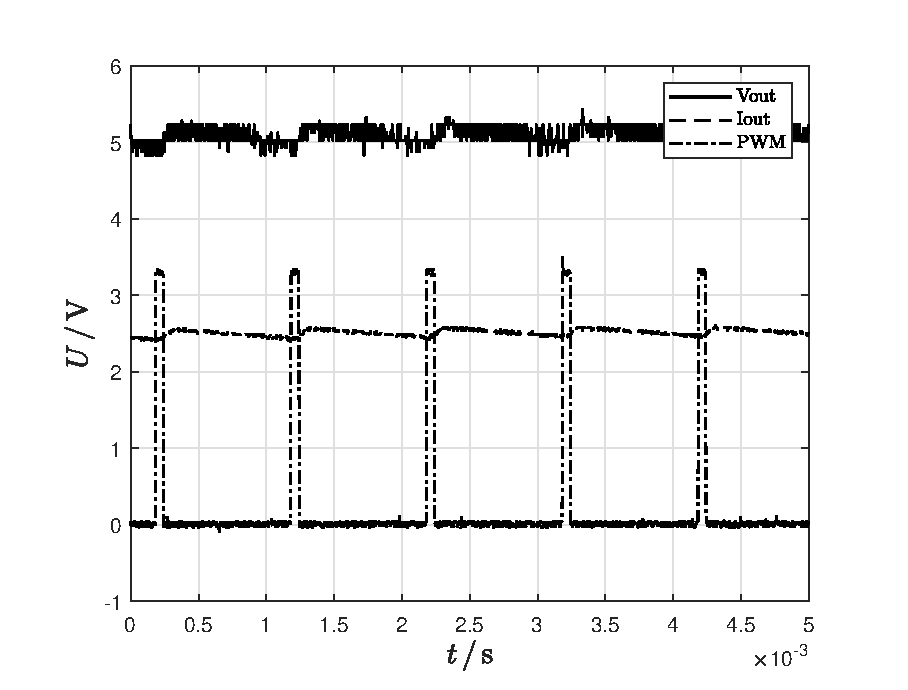
\includegraphics[width=0.8\linewidth]{Figure/Rload2.eps}
    \caption{Messung mit $R_{load} = \SI{2}{\ohm}$}
    \label{fig:Rload2}
\end{figure}

\begin{figure}[H]
    \centering
    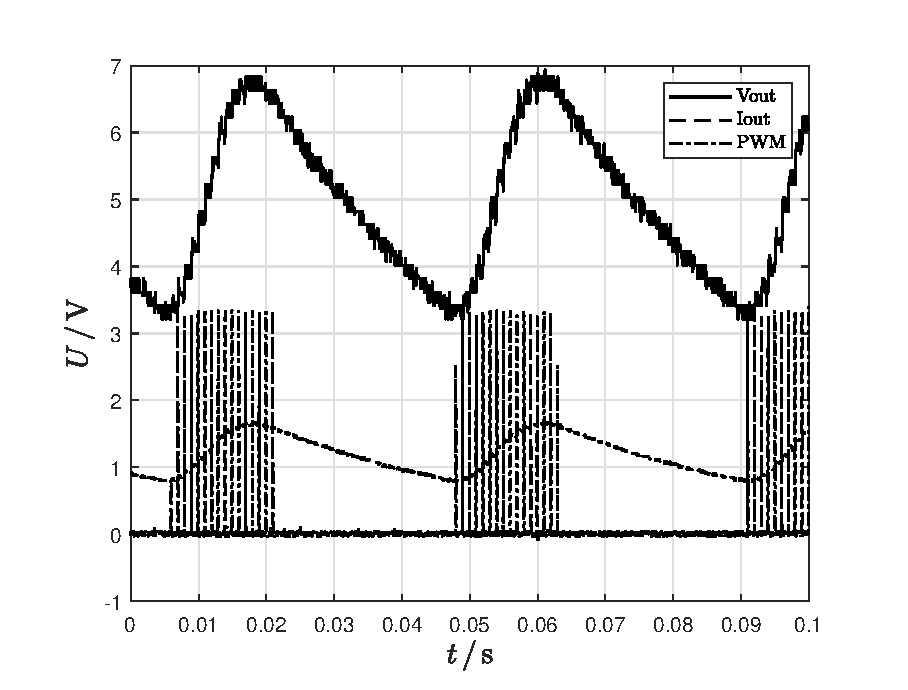
\includegraphics[width=0.8\linewidth]{Figure/Rload4.eps}
    \caption{Messung mit $R_{load} = \SI{4}{\ohm}$}
    \label{fig:Rload4}
\end{figure}